\vspace{3cm}

% \begin{center}
%     \textbf{Àlex Giménez-Romero$^{1}$, Federico Vázquez$^{2,1}$, Cristóbal
%         López$^{1}$, Manuel A. Matías$^{1}$}
% \end{center}

% \vspace{1cm}

% \begin{enumerate}
%     \small
%     \item Instituto de Física Interdisciplinar y Sistemas Complejos, IFISC
%           (CSIC-UIB), Palma de Mallorca 07122, Spain
%     \item Instituto de Cálculo, FCEyN, Universidad de Buenos Aires and CONICET,
%           Buenos Aires, Argentina

% \end{enumerate}

% \vspace{1cm}

\textbf{Published as}

\vspace{0.5cm}

\fullcite{GimenezRomero_2022_RSos}

\newpage
\section{Introduction}

Wildlife emergent infectious diseases represent a substantial threat to
ecosystems and the conservation of their biodiversity \cite{Daszak443}. Their
effects can be devastating at the ecological level, causing local extinctions
\cite{Daszak443} and in some cases pushing endemic species to the verge of
extinction, as is the case of \textit{Pinna nobilis}
\cite{Cabanellas2019}; at the economic level, producing losses in agriculture,
livestock and aquaculture \cite{Vurro2010, Tomley2009, Pernet2016}, and impact
human health, as is the case of the COVID-19 pandemic \cite{Salata2020}. For
the past decades, parasites have been continuously emerging \cite{Morens2004,
    Daszak2017}, while globalisation and climate change have contributed to
their
evolution. This has allowed these parasites to enter in new ecological niches
and spread further the diseases they produce \cite{Aguirre2008}. In particular,
marine infectious diseases are recently increasing due to these and other
anthropogenic pressures, like pollution and overfishing \cite{Lafferty2004},
inducing widespread mass mortalities in several species \cite{Eisenlord2016,
    JONES201648, VAZQUEZ2017}.

An important subset of marine organisms affected by infectious diseases are
sessile (i.e. they cannot move), like bivalves, sponges or corals. An
increasing number of outbreaks affecting marine mollusks have been reported,
some of them causing mass mortalities in commercially important bivalves
\cite{Guo2016}. Mainly due to the economic importance of some species (e.g.
oysters), infectious diseases in bivalve populations have been deeply studied
\cite{Petton2021, Pernet2018, McLaughlin2005, powell1999modeling}. Recently,
deterministic compartmental models have been used to describe parasite
transmitted diseases in marine sessile bivalves \cite{BIDEGAIN_2016_2,
    BIDEGAIN_perkinsus, GimenezRomero2021}, showing to be able to accurately
predict disease transmission in some circumstances. The main limitation of
these compartmental models is the assumption of a non-spatial description of
the system under study. This underlying hypothesis assumes that any pair
parasite-host of the system can interact at any time, which is unrealistic in
general. A non-spatial description assumes well mixed populations, which
implies that the mean distance among hosts is smaller than the the typical
distance explored by parasites in their lifetime. This assumption can be quite
realistic in some situations, as it is in \cite{GimenezRomero2021} where the
hosts were kept in tanks with water renovation. However, a non-spatial model is
not expected to yield a good description of spatially extended hosts in a
natural setting.

The key quantity in mathematical epidemiology is the basic reproductive number,
$R_0$, that represents the number of infected individuals generated in one
generation by the appearance of a single infected individual in a fully
susceptible population. Thus, $R_0>1$ ensures the onset of an epidemic, as the
number of infected individuals will grow exponentially	producing a widespread
disease \cite{Anderson1991}. If we first disregard spatial effects and assume a
non-spatial description, $R_0$ can be obtained from standard methods, like the
Next Generation Matrix method \cite{Diekmann2010}, and will only depend on
\textit{intrinsic} characteristics of the pathosystem (host-pathogen system)
under study. However, this basic reproduction number is unable to characterise
the threshold behaviour in many situations, including spatially extended
systems \cite{Cross2007, Li2011, RILEY201568}. In these systems, the
propagation of an epidemic to the entire system needs that a certain spatial
threshold is exceeded \cite{Gilligan2008}. Otherwise the disease will only take
place in suitable localised parts of the system, not being able to propagate to
the total system. Thus, disease spread will be strongly affected by the host
spatial distribution and pathogen mobility, which are not accounted for in
non-spatial models.

In this work we will try to unravel the transmission mechanisms of a
parasite-induced disease affecting immobile hosts in a spatially extended
system. We will approach the problem both theoretically and through numerical
simulation. The numerical study is based on Individual-Based Modelling (IBM), a
method widely used to study ecological systems \cite{Grimm2005}, so that
individuals are treated as discrete entities, space is introduced explicitly
and the dynamics are stochastic. Representative average behaviours can be
obtained by averaging over a sufficient number of realisations, and the
accuracy of the approach can be calibrated by deriving the corresponding
non-spatial limit, that can be confronted with the suitable compartmental model
on which a particular IBM is based. The IBM approach to our problem will allow
to study in depth the relation between pathogen mobility and immobile host
infection. As parasites move randomly over the space, tracking the position of
each parasite at different times turns to be of fundamental importance to
properly capture the stochastic dynamics of infections from parasites to hosts.
Modelling parasites and hosts as individual entities allows to take into
account the spatial and temporal heterogeneity of interactions between them.
This heterogeneity and the level of control in microscopic interactions cannot
be captured by other mathematical approaches such as partial differential
equations. On the other hand, IBMs are mathematically involved, and analytical
treatments are normally cumbersome, while their numerical implementation is
computationally expensive \cite{Breckling1900}.

Here we introduce a spatially-explicit individual-based model to study
parasite-induced marine diseases of immobile hosts. The model is applied  to
the case of diffusing parasites and uniformly distributed hosts. The system
under study is an extension of the compartmental model presented in
\cite{GimenezRomero2021}. As a main result, we find that the occurrence of an
outbreak will depend on the balance between the intrinsic characteristics of
the pathosystem, well represented by the above described non-spatial basic
reproductive number, $R_0$, and features that characterise parasite mobility.
We generalise the basic reproductive number, that we will refer to as
$\tilde{R}_0$, such that it accounts for the number of hosts that get infected
by the appearance of a single infected individual in a fully susceptible
population in a spatially extended system. $\tilde{R}_0$ characterises the
global epidemic and can be written as a product between $R_0$ and a factor
describing parasite mobility. The latter factor is smaller and at most equal to
$1$, which implies that, as it could be expected, it is more difficult to
induce a global outbreak in a spatially extended system (a two dimensional
lattice in our case) that in a well mixed (non-spatial) population.

% The paper is organised as follows: in \cref{sec:model}, we introduce some
% biological considerations for bivalve epidemics, discussed in more detailed in
% Ref. \cite{GimenezRomero2021}, and build the spatially-explicit model. In
% \cref{sec:results}, we present analytical results that are discussed and
% supported by numerical simulations. Specifically, the high mobility limit is
% discussed and connected to the the compartmental model. An approximation for
% the parasite population is discussed. Then, the effect of parasite mobility to
% the epidemic threshold is characterised, deriving an analytical expression for
% the basic reproduction number. Furthermore, the spreading speed of the disease
% and the time-scale to extinction is investigated. Finally, \cref{sec:
%     conclusions} contains some concluding remarks.

\section{The SIRP spatial model} \label{sec:model}

The most important biological features of the system under study are as
follows. First, hosts are immobile, while the disease is transmitted by
parasites produced by infected hosts. There are two mechanisms by which
parasites are cleared from the medium: i) they have a finite life time after
which they die or get inactivated; ii) they get absorbed after they infect a
host and thus are no
longer in the medium and cannot infect other hosts. Recruiting (birth) of hosts
occur at a very slow rate compared to other timescales in the system, and
accordingly it will be considered negligible in the model. Moreover, hosts do
not show long-term immunity, as is typical of invertebrates, like mollusks
\cite{Powell2015}. We also assume that recovery (healing) of infected hosts, if
it occurs, can be neglected. Furthermore, we consider that dead hosts are not a
source of parasites in the medium. See \cref{ch:nacras_I}
\cite{GimenezRomero2021} for a detailed
presentation of the non-spatial SIRP model, including these biological
modelling considerations.

Under these considerations, we introduce an individual-based model with
explicit space characterisation to study the effect of parasite mobility in
disease transmission. We consider a square grid of length $L$ with periodic
boundary conditions and place a single host per site, so that there are $N=L^2$
hosts. The hosts can be in three discrete states: susceptible, $S$; infected,
$I$ and dead (or removed), $R$. Then, we introduce the parasite population as a
new individual with a single state, $P$. Hosts are sessile (i.e. immobile),
while parasites are allowed to move between the lattice sites. As initial
condition we assume that the entire host population is susceptible,
$S(0)=N=L^2$, and that a small initial number of parasites, $P(0)$ is
introduced in the system.

Infection occurs when susceptible hosts filter parasites in their close
proximity. Accordingly, the infection process is implemented between parasites
and susceptible hosts sharing the same lattice site. In particular, susceptible
hosts in contact with a parasite become infected at rate $\beta$. As the
infection event implies the filtering of a parasite by a susceptible host, when
a new infection occurs a parasite of that particular site is removed. Infected
individuals die at rate $\gamma$ and produce parasites at rate $\lambda$, while
parasites die at rate $\mu$. Parasites move randomly between the four
neighbouring lattice sites at rate $\kappa$, which corresponds to a diffusive
motion. \cref{tab:IBM_params} contains the definitions of the variables and
parameters of the model and \cref{fig:IBM} shows a schematic representation of
the dynamics.

\begin{figure}[H]
    \centering
    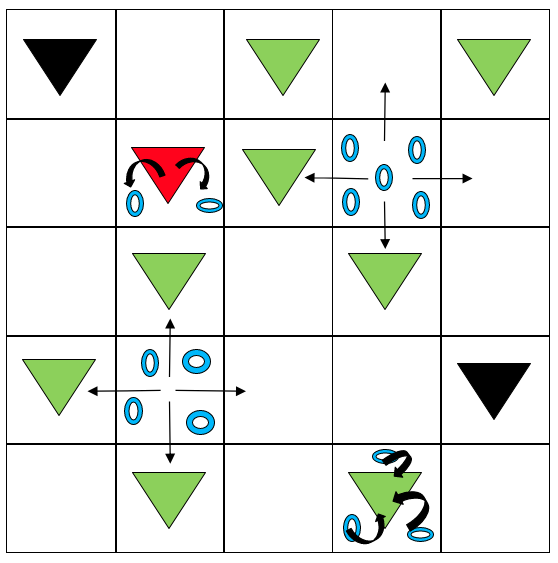
\includegraphics[width=0.6\textwidth]{Figures/IBM.png}
    \caption[Scheme of the individual based SIRP model]{Scheme of the
        individual based model. Green, red and black
        triangles represent susceptible, infected and dead hosts, respectively.
        Blue
        rings represent parasites, which move randomly between cells.
        Susceptible hosts
        get infected by filtering parasites while infected hosts produce them.
        Dead
        hosts do not participate in the dynamics of the system.}
    \label{fig:IBM}
\end{figure}

\begin{table}[H]
    \centering
    \caption[Variables and parameters of the individual based SIRP
        model]{Variables and parameters of the individual based SIRP model.}
    \resizebox{0.8\columnwidth}{!}{
        \begin{tabular}{cl}
            \hline \hline
            \textbf{Variable/Parameter} & \textbf{Definition}
            \\ \hline
            S                           & Susceptible host
            \\
            I                           & Infected host
            \\
            R                           & Dead host
            \\
            P                           & Parasite
            \\
            $\beta$                     & Parasite-host transmission rate
            \\
            $\gamma$                    & Host mortality rate
            \\
            $\lambda$                   & Production rate of parasites by
            infected hosts
            \\
            $\mu$                       & Parasite natural death rate
            \\
            $\kappa$                    & Parasite dispersal rate (mobility)
            \\
            $R_0$                       & Non-spatial basic reproductive number
            \\
            $\tilde{R}_0$               & Spatial basic reproductive number
            \\ \hline \hline
        \end{tabular}
    }
    \label{tab:IBM_params}
\end{table}

Formally, the model is mathematically described by a system of $N$ master
equations for the probabilities of the states in each lattice site $i$.
\cref{eq:scheme} summarises the reactive events. This is
very difficult to manage analytically, so the time evolution of the model is
numerically solved using Gillespie's algorithm \cite{Gillespie1977} (the code
can be found in \cite{CODE_nacras}).
\begin{equation}\label{eq:scheme}
    S+P \stackrel{\beta}{\rightarrow} I + \varnothing \quad I
    \stackrel{\gamma}{\rightarrow} R \quad I \stackrel{\lambda}{\rightarrow}
    I+P
    \quad P \stackrel{\mu}{\rightarrow} \varnothing
\end{equation}

\section{Results}\label{sec:results}
In this section several features of the model are studied, both numerically
(from IBM simulations) and analytically. All numerical results were obtained
for a square lattice of length $L=100$, with $N=S(0)=10^4$ hosts and using a
small initial condition of $P(0)=50$ parasites in the centre site.

\subsection{Non-spatial limit} \label{sec:MFlimit}
An important test of the IBM implementation is to show that, under suitable
circumstances, it converges to the non-spatial model on which the IBM is based.
This occurs in the limit when the parasites move many times before dying or
infecting a susceptible host. In this situation, each parasite typically visits
all the hosts of the system and may infect any of them. This is equivalent to
infecting a random host of the system, which happens with probability $\beta
    S/N$, being $S$ the total number of susceptible hosts in the system.
This corresponds to standard incidence, which represents the most accurate
description of the infection process
(\cref{ch:nacras_I},\cite{GimenezRomero2021}).
An equivalent picture is that parasites will end up uniformly distributed in
the lattice, so that there will be $P/N$ parasites in each lattice site at any
time. One expects to reach these conditions when $\kappa\gg\mu,\beta$, and,
thus the system as a whole can be described by the following system of ordinary
differential equations (ODE's),
\begin{equation}\label{eq:SIRP_MF}
    \begin{aligned}
        \dot{S} & =-\beta P S/N \, ,               \\
        \dot{I} & =\beta P S/N-\gamma I \, ,       \\
        \dot{R} & =\gamma I \, ,                   \\
        \dot{P} & =\lambda I-\beta P S/N-\mu P \ ,
    \end{aligned}
\end{equation}
that is precisely the SIRP non-spatial model \cite{GimenezRomero2021}, where
$S$, $I$, $R$ are the total number of susceptible, infected and recovered hosts
in the system, $P$ the total number of parasites and $N$ is the number of
hosts.

The basic reproduction number, $R_0$, of this non-spatial model is the
dimensionless quantity that yields the number of secondary infections generated
by the appearance of a single infected individual in a completely susceptible
population, also indicating whether the system will exhibit an epidemic
outbreak, $R_0>1$, or not, $R_0<1$.
In our case it can be directly computed as the mean number of parasites
produced by an infected host during its mean lifetime, $\lambda/\gamma$, times
the mean number of susceptible hosts that get infected by parasites during
their mean lifetime, $\beta/(\mu+\beta)$,
\begin{equation}\label{eq:R0_MF}
    R_0=\frac{\lambda}{\gamma}\frac{\beta}{\mu+\beta} \ .
\end{equation}
This result can be corroborated with standard methods such as the Next
Generation Matrix method \cite{Diekmann2010} (see \cite{GimenezRomero2021}),
where $S(0)=N$ has been considered.

Moreover, the model has a conserved quantity $\mathcal{C}$
\cite{GimenezRomero2021} that allows to find an analytical expression for the
final number of dead individuals (\cref{app:Rinf}),
\begin{equation}\label{eq:R_inf}
    R(\infty)=N+\frac{S(0)}{\xi}W_0\parentesi{-\xi\exp(-\frac{\beta}{\mu}C)} \
    ,
\end{equation}
with $\displaystyle\xi=S(0)\frac{\beta\parentesi{\lambda-\gamma}}{\mu\gamma}$
and $\displaystyle C=P_0+\frac{\lambda}{\gamma}\parentesi{S(0)+I(0)}-S(0)$.

The non-spatial limit of the model has been evaluated by comparing realisations
of the stochastic model (in the limit $\kappa\gg\mu,\beta$) with numerical
solutions of the non-spatial ODE system of \cref{eq:SIRP_MF}. Furthermore, the
analytical expression for $R(\infty)$ using the non-spatial model,
\cref{eq:R_inf}, is also compared to the numerical results of the individual
based model. As shown in \cref{fig:MF_limit} (a)-(c), as $\kappa$ is increased
compared to $\mu$ the individual based model approaches the non-spatial one.
\cref{fig:MF_limit}(d) shows how the numerical results for $R(\infty)$ for
different $R_0$ values approach the analytical solution in the non-spatial
limit.

\begin{figure}[H]
    \centering
    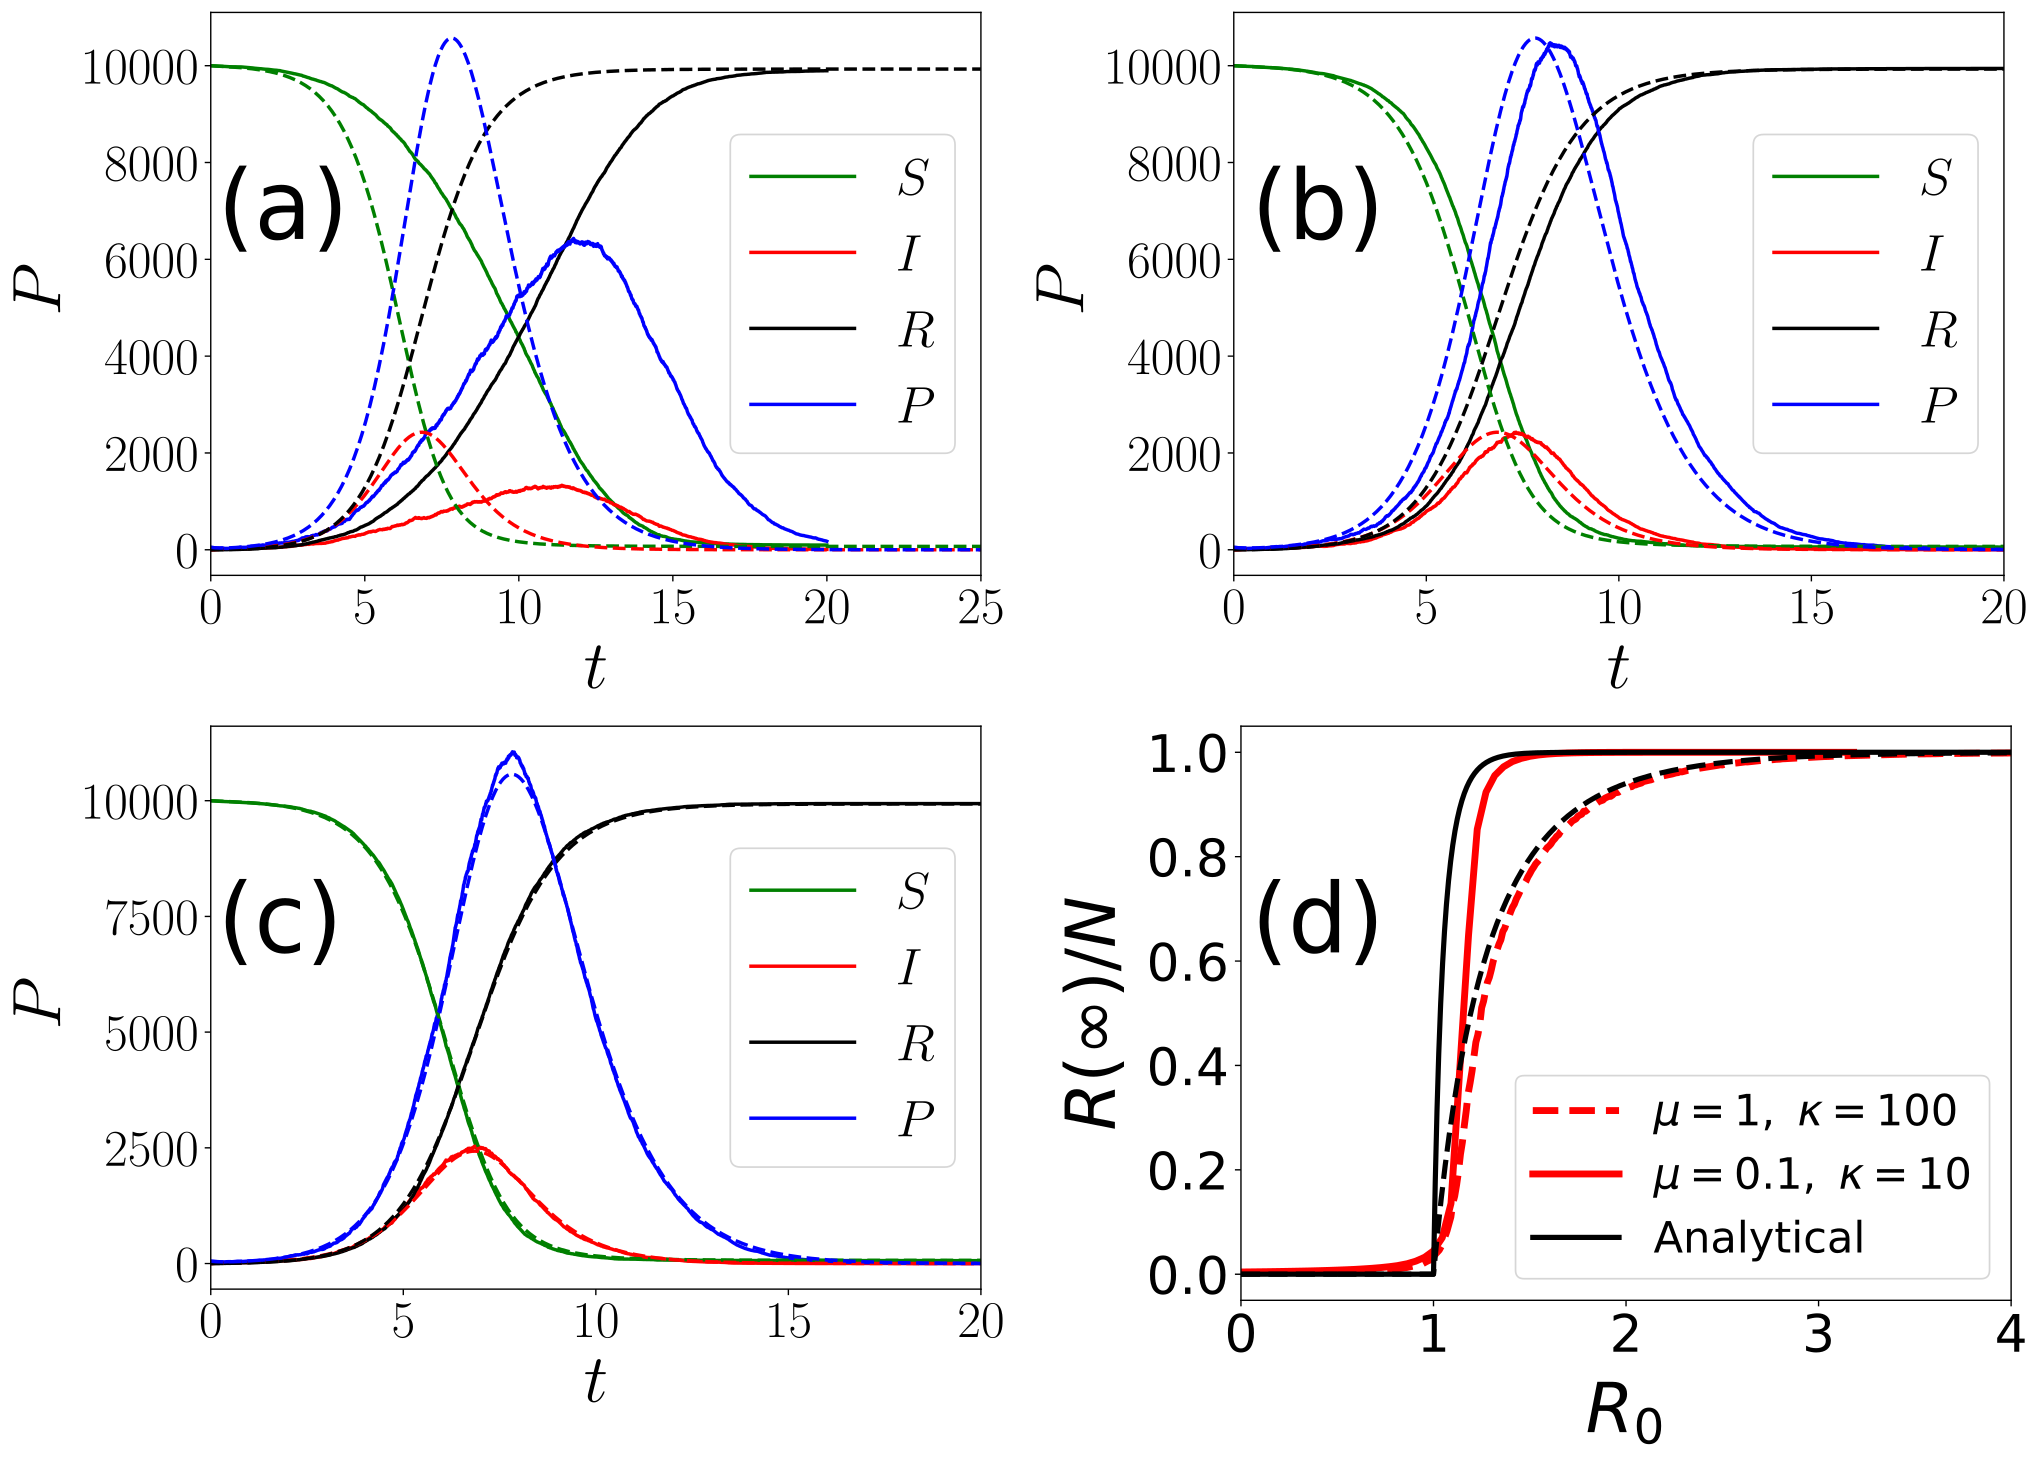
\includegraphics[width=\columnwidth]{Figures/MF_comparison.png}
    \caption[
        Comparison between the non-spatial model and the individual based model
        in the high mobility limit
    ]{Numerical solution of the non-spatial model (\cref{eq:SIRP_MF},
        dashed lines) compared with numerical solutions of the individual based
        model
        (solid lines) approaching the non-spatial limit with fixed
        $\gamma=\mu=\beta=1$
        and $\lambda=6$. (a) $\kappa=10^2$, (b) $\kappa=10^3$, (c)
        $\kappa=10^4$. Panel
        (d) shows the final fraction of dead hosts, $R(\infty)/N$, as function
        of $R_0$
        for $\kappa/(\mu+\kappa)=0.999$ with $\mu=1,0.1$ compared to the
        analytical
        result.}
    \label{fig:MF_limit}
\end{figure}

\subsection{Approximate relation between parasites and infected hosts}

In the limit $\kappa\gg\beta,\mu$ a time-scale approximation can be
performed so that the parasite population dynamics directly relates to that of
the infected hosts. In the non-spatial limit it was already shown in
\cite{GimenezRomero2021} that, if  $\mu\gg\beta,\gamma$ and $\lambda\gg\beta
    P/N$, the total parasite population of the system can be well described
using
the approximation (see \cite{GimenezRomero2021} for a detailed discussion),
\begin{equation}\label{eq:P_approx_II}
    P(t)\approx \frac{\lambda}{\mu} I(t) \ .
\end{equation}

Here we extend the validity of this approximation to spatial systems far
from the non-spatial limit. Consider the local dynamics of the parasite
population on a lattice site $i$. Note that when the host in the site is
susceptible, parasites in this site can either infect the host, die, or move to
another site. All these processes imply that a parasite will disappear from the
current site. Once the host at site $i$ gets infected, infection can no longer
occur whereas parasite production is now possible. If $\kappa$ is small enough
compared to $\lambda$ and $\mu$,  the only competing processes in sites with
infected individuals will be the production of parasites and their natural
death, which can be fairly described by the following rate equation,
\begin{equation}
    \der{P}{t}=\lambda-\mu P \ ,
\end{equation}
which solution is
\begin{equation}\label{eq:P_evol}
    P(t)=\frac{\lambda}{\mu}+\claudator{P(0)-\frac{\lambda}{\mu}}e^{-\mu t}
    \ .
\end{equation}

From \cref{eq:P_evol} one may notice that the stationary value of $P$,
$\lambda/\mu$, is reached in a time proportional to $t_{\textrm{eq}}\propto
    1/\mu$. This derivation allows to find a condition for which
\cref{eq:P_approx_II}
is valid beyond the non-spatial limit. Basically, if the mean dispersal time,
$1/\kappa$, is greater than the equilibrium time, $t_{\textrm{eq}}\propto
    1/\mu$, parasites in sites with infected hosts will reach its stationary
level
before parasites enter or leave the sites. Thus, sites with infected hosts can
be considered as a closed system and the approximation holds. In other words,
if the dispersal rate of parasites is small compared to the parasite
deactivation rate, $\kappa \ll \mu$, the local parasite population of the site
will reach its stationary level $P_i=\lambda/\mu$. It is possible to extend the
result to the entire system: if there are $I(t)$ infected sites in the system
at time $t$ and $\kappa\ll\mu$ is fulfilled, there will be a total parasite
population of $P(t)=(\lambda/\mu) I(t)$, which is equivalent to
\cref{eq:P_approx_II}.

\begin{figure}[H]
    \centering
    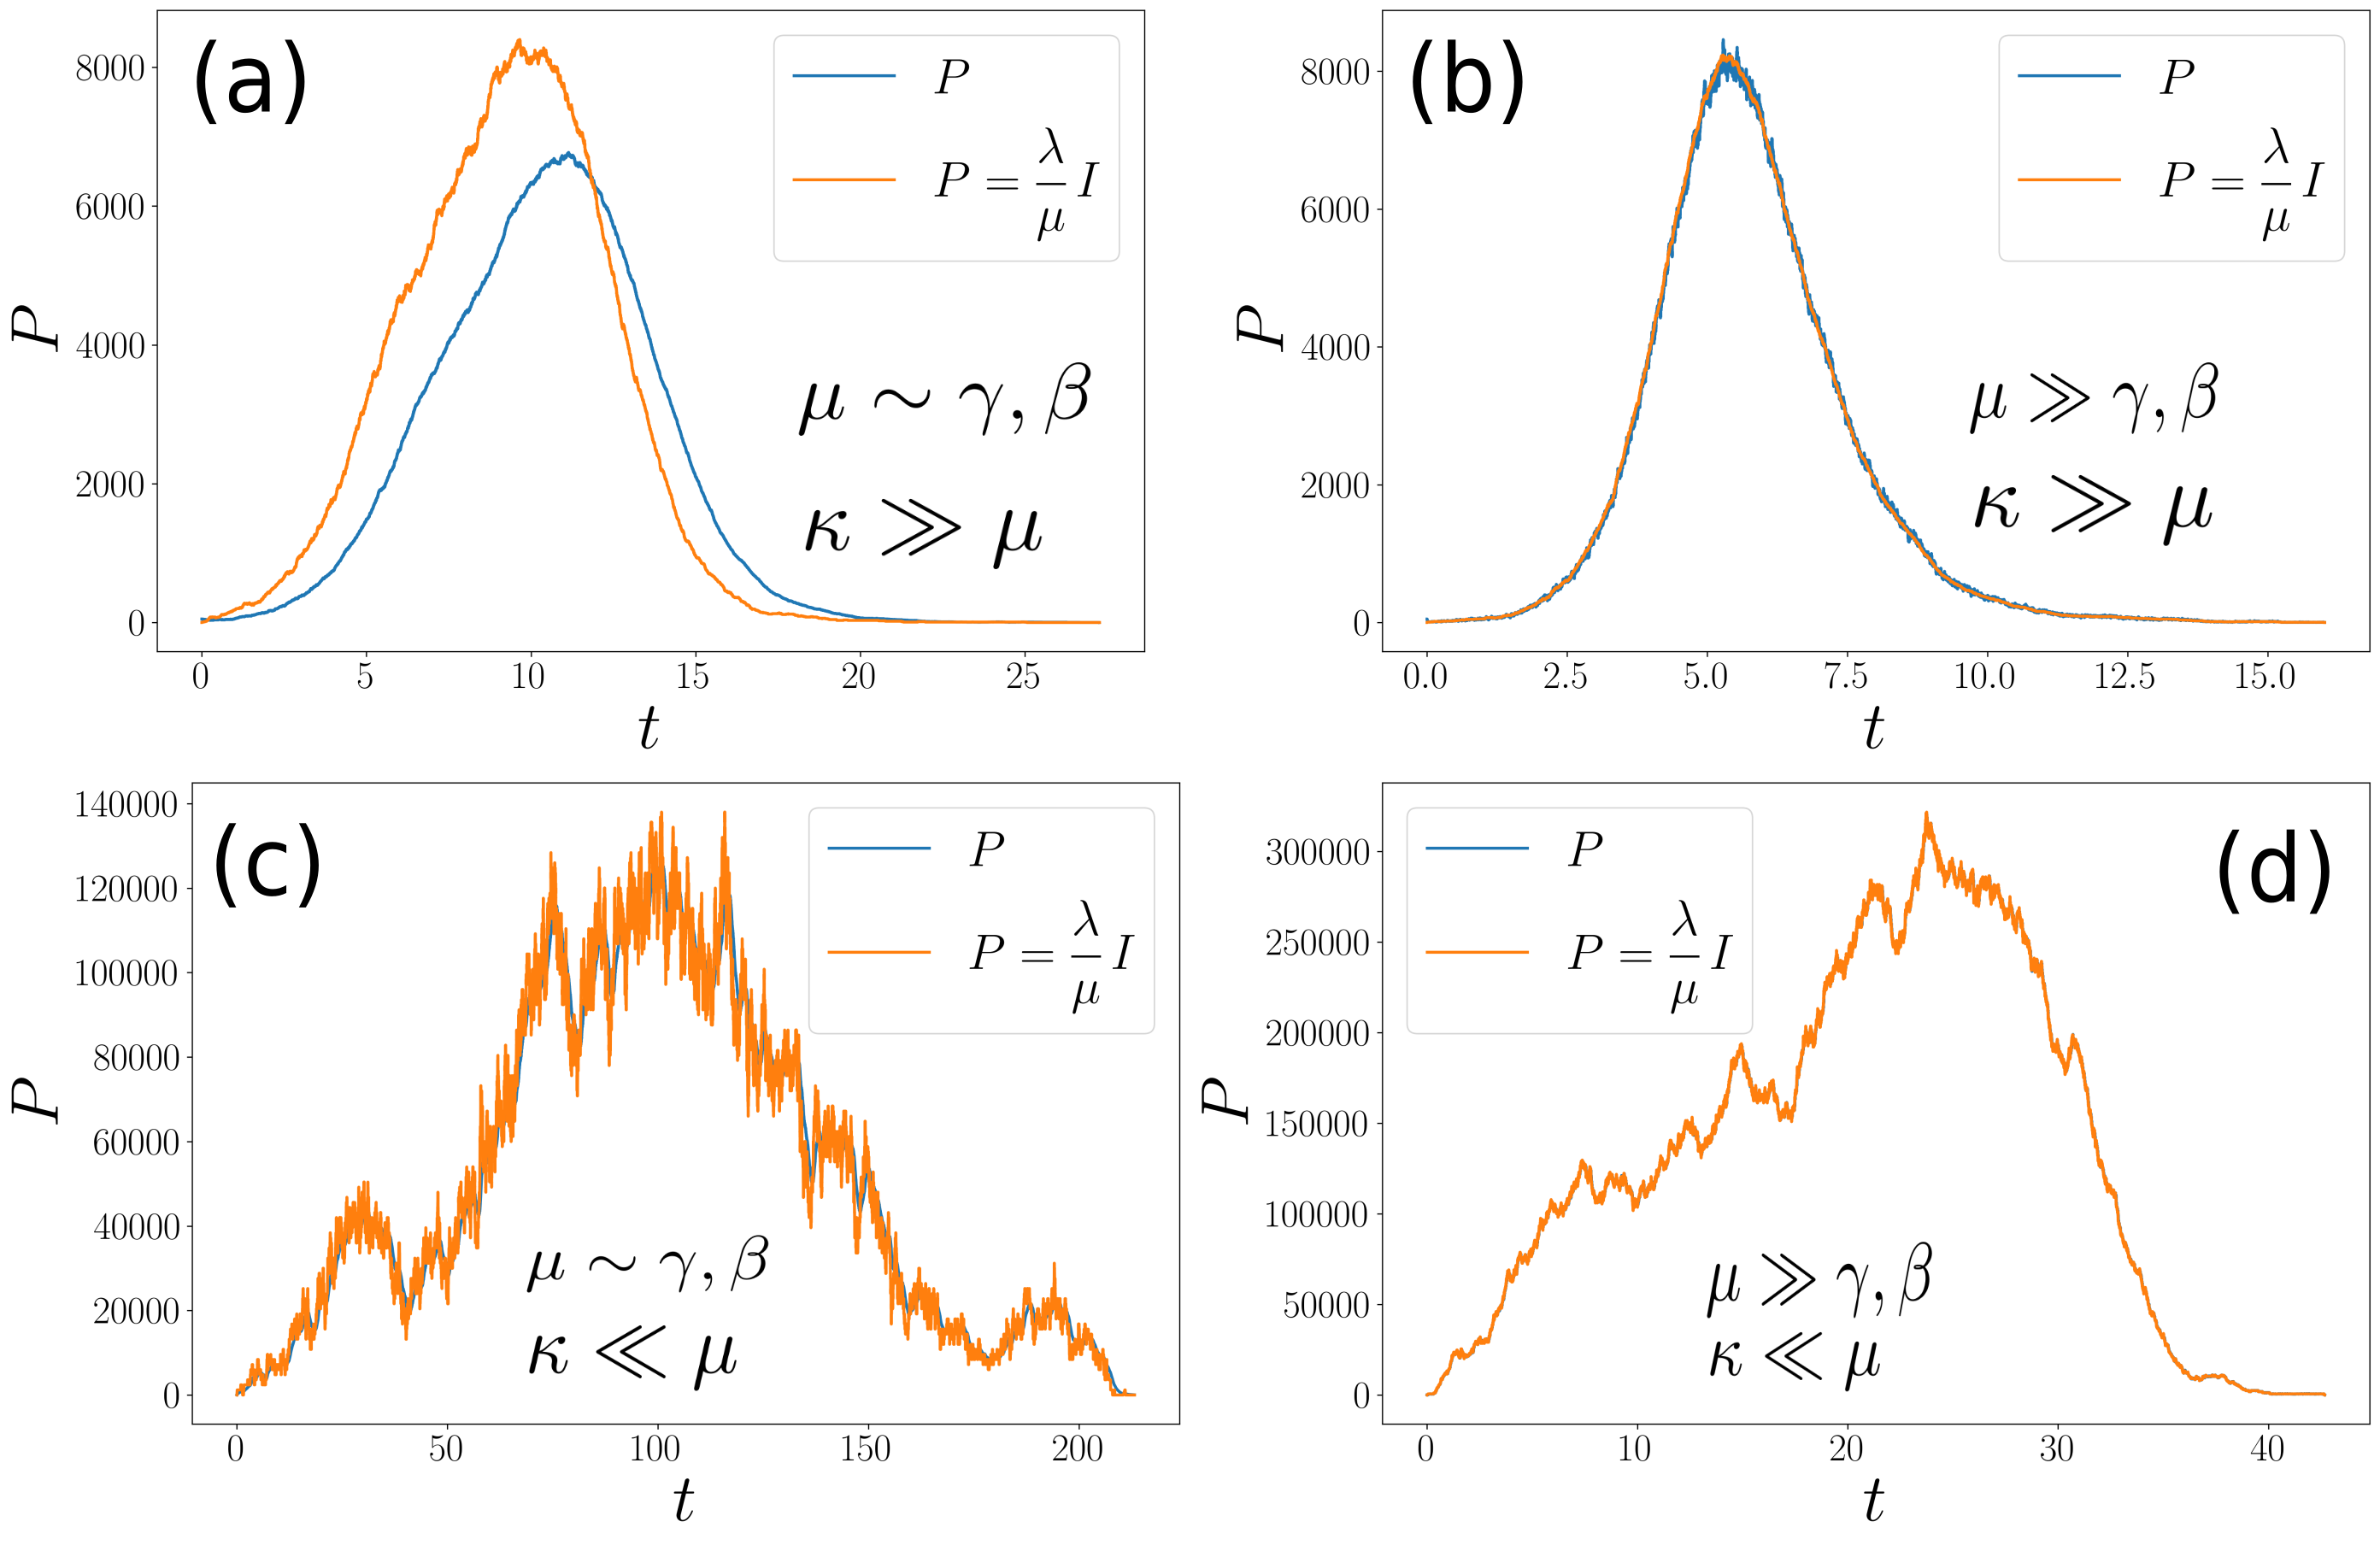
\includegraphics[width=\columnwidth]{Figures/P_approx.png}
    \caption[Validation of the approximate expression for the parasite
        population dynamics]{Numerical verification of the approximate
        expression for the parasite population dynamics, \cref{eq:P_approx_II},
        for different mobility conditions. The simulations were performed
        fixing $\beta=\gamma=1$ for all panels. (a) $\mu=1$ $\kappa=10^2$,
        $\lambda=6.06$, $\kappa/(\mu+\kappa)=0.99$;
        (b) $\mu=100$, $\kappa=10^4$, $\lambda=306$,
        $\kappa/(\mu+\kappa)=0.99$; (c)
        $\mu=1$, $\kappa=0.01$, $\lambda=1200$, $\kappa/(\mu+\kappa)=0.01$; (d)
        $\mu=100$, $\kappa=1$, $\lambda=60600$,  $\kappa/(\mu+\kappa)=0.01$}
    \label{fig:P_approx}
\end{figure}

Thus, for the non-spatial limit ($\kappa\gg\mu$) we have that if
$\mu\gg\beta,\gamma$ \cref{eq:P_approx_II} is valid, while for $\kappa\ll\mu$
the
approximation is also valid regardless of the value of $\beta,\gamma$, as the
nature of the approximation is different. Thus, in general, as $\kappa$
decreases over $\mu$ (the lower the parasite mobility becomes) we expect the
approximation to work better.

The parasite approximation to infected hosts dynamics, \cref{eq:P_approx_II},
is numerically verified for different mobility conditions.
\cref{fig:P_approx}(a)-(b) shows how the approximation improves as $\mu$ grows
over $\beta,\gamma$ (mean errors are $0.18$ and $0.0081$, respectively) in the
non-spatial limit, i.e. $\kappa\gg\mu$, as expected. This result is in perfect
agreement with that found in \cite{GimenezRomero2021}. Then,
\cref{fig:P_approx}(c)-(d) show that the approximation is valid in general when
$\kappa\ll\mu$ but improves anyway when $\mu\gg\beta,\gamma$ (mean errors are
0.04 and 0.0026, respectively). Summarising, we see that the lower the value of
$\kappa$ is with respect to $\mu$ the more valid \cref{eq:P_approx_II} is,
regardless of the value of $\beta,\gamma$, while in the non-spatial limit,
$\kappa\gg\mu$, the condition $\mu\gg\beta,\gamma$ is needed.

\subsection{Spatial threshold}

One of the main questions in epidemiology is to define the conditions under
which an epidemic outbreak occurs, which usually is translated into the
existence of a threshold. In a well mixed (non-spatial) system the basic
reproduction number ($R_0$), that characterises this threshold $R_0=1$, can be
defined exclusively from \textit{intrinsic} parameters of the pathosystem, as
the host-pathogen interaction does not depend on the host spatial structure or
pathogen mobility (see \cref{eq:R0_MF}). In stochastic spatial models this
formulation of $R_0$ breaks down. First of all, in stochastic models, even
above the threshold there is a non-zero probability that the disease is unable
to propagate initially, given by
$P_{\textrm{outbreak}}=1-\parentesi{1/R_0}^{I(0)}$ \cite{Brauer2008}.
Furthermore, the discrete nature of the populations also modifies the estimates
of $R_0$ \cite{KEELING200051}. On the other hand, the introduction of space
changes completely the nature of epidemic outbreaks, modifying the
host-pathogen interactions by means of specific host spatial distributions and
pathogen mobility patterns. Even if the basic reproduction number of the
non-spatial model is above the threshold ($R_0>1$), if parasite mobility is not
large enough, the epidemic will stay locally confined. Thus, one expects that
the threshold at which an epidemic outbreak can propagate to the rest of the
system will depend on the balance between the intrinsic pathosystem parameters
in $R_0$ and parasite mobility, defining a spatial basic reproduction number,
$\tilde{R}_0$.

Having in mind the study in \cref{sec:MFlimit}, we expect that in the high
mobility limit the basic reproduction number is defined by the non-spatial
formula, \cref{eq:R0_MF}. On the other hand, the lower the parasite mobility
is, the more difficult will be for a local outbreak to propagate through the
system. Thus, it is natural to think of an spatial basic reproduction number of
the form $\tilde{R}_0=R_0 f(\kappa)$, where $f(\kappa)$ is an increasing
function of the parasite dispersal rate accounting for parasite mobility
fulfilling $\lim_{\kappa\to\infty}f(\kappa)=1$.

Indeed, some authors recently showed that the spatial basic reproduction
number can be defined as the product between the non-spatial value, $R_0$, and
a factor accounting for spatially-dependent interactions, $f(r)$, in the form
$\tilde{R}_0=R_0f(r)$ \cite{Filipe2003,Filipe2004,Gilligan2021}. However, these
expressions are not analytical \cite{Filipe2003,Filipe2004} or are not directly
related to pathogen mobility \cite{Gilligan2021}. Here we propose a simple
expression for the spatial basic reproduction number regulating the spatial
propagation of the epidemic,
\begin{equation}\label{eq:R_0ibm}
    \tilde{R}_0=\frac{\lambda}{\gamma}\frac{\beta}{\mu+\beta}
    \frac{\kappa}{\mu+\kappa}=R_0\frac{\kappa}{\mu+\kappa}
    \ .
\end{equation}

The derivation of \cref{eq:R_0ibm} accounts for the number of secondary
parasites that are able to produce new infections, or equivalently, the number
of secondary infections produced by an initial infected host. If we consider an
initial infected individual, on average it will produce $\lambda/\gamma$
parasites. Then, these parasites can only move to neighbouring sites or die, so
that the dispersal probability is given by $\kappa/(\mu+\kappa)$. Finally,
considering that parasites do not affect each other trying to infect the same
host, the infection probability is given by $\beta/(\mu+\beta)$. Joining all
terms, we finally obtain \cref{eq:R_0ibm}. This expression is valid when
parasites move only to sites with susceptible individuals and do not try to
infect the same host. Thus, the derived $\tilde{R}_0$ is only an approximation
to the spatial basic reproduction number for the case of an initial
introduction of a small quantity of parasites in a fully susceptible
population.

Note that, as expected, the spatial basic reproduction number is nothing
other than the basic reproduction number of the non-spatial model multiplied by
an increasing function of the parasite mobility, $\kappa/(\mu+\kappa).$ Taking
the limit $\kappa\gg\mu$ in \cref{eq:R_0ibm} (non-spatial limit) the basic
reproduction number of the non-spatial model is recovered. Conversely, in the
limit of very low mobility, the $\kappa/(\mu+\kappa)$ factor is small, and this
has to be compensated with a large value of the non-spatial basic reproduction
number, $R_0$, in order that there is an outbreak, i.e., $\tilde{R}_0>1$.

The spatial threshold, $\tilde{R_0}=1$, given by \cref{eq:R_0ibm}, has been
numerically checked by computing the phase diagram between the absorbing phase
$R(\infty)\approx 0$ (no infection, i.e. disease-free state)  and the active
phase $R(\infty)> 0$ (in which some level of infection has occurred, i.e.
propagation phase) for several values of the parasite mobility and the basic
reproduction number of the non-spatial model, $R_0$ \cref{eq:R0_MF}. The
transition is expected to occur at $\tilde{R}_0=1$, implying from
\cref{eq:R_0ibm} that the dependence of the critical value of $R_0$, say
$R_0^c$, is expected to take the form,
\begin{equation}\label{eq: R_0_crit dependence}
    R_0^c\sim\parentesi{\frac{\kappa}{\mu+\kappa}}^{-1} \ .
\end{equation}
As discussed above, we expect that $\tilde{R}_0=1$ with $\tilde{R}_0$ given
by \cref{eq:R_0ibm} does not represent exactly the spatial threshold, and for
this reason we suggest the more general functional form,
\begin{equation}\label{eq: threshold_corrections}
    R_0^c\sim A\parentesi{\frac{\kappa}{\mu+\kappa}}^{-B} - C\ ,
\end{equation}
to be be fitted to numerical data, where $A=1$, $B=1$ and $C=0$ would imply
a perfect agreement of numerical simulations of the IBM model with
\cref{eq:R_0ibm}.

In order to obtain the phase diagram, we compute the absorbing state of the
model as an average over $1000$ realisations for each value of the mobility and
$R_0$ considered. Then, the critical value $R_0^c$ is computed for each
mobility value as the $R_0$ value for which the fluctuations of the ``order
parameter'' $\displaystyle \chi=\avg{{R(\infty})^2}-\avg{R(\infty)}^2$ are
maximal, as this would be an indication of a transition between the
disease-free and the propagation phases.

\begin{figure}[H]
    \centering
    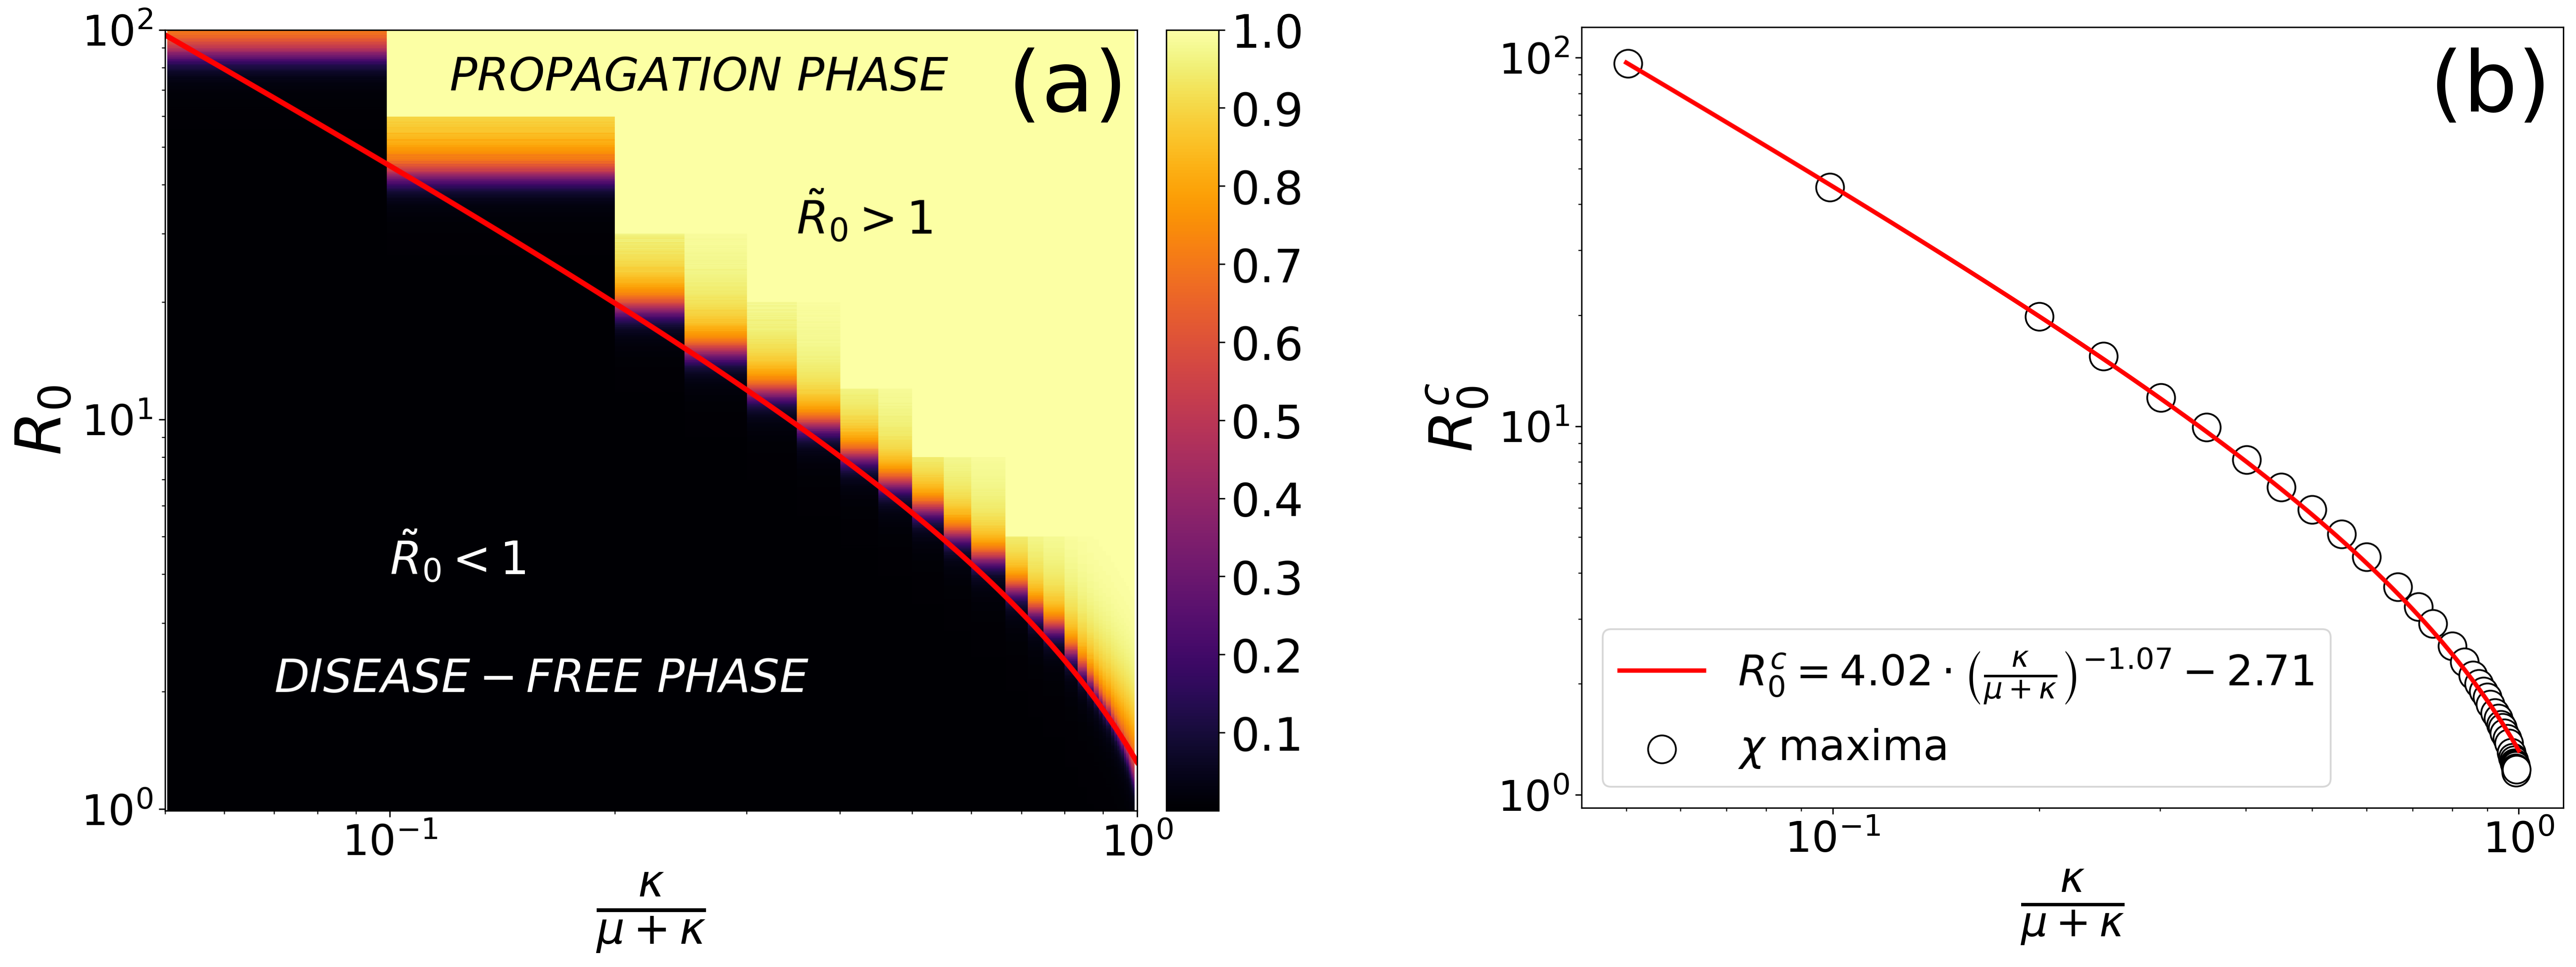
\includegraphics[width=1\textwidth]{Figures/PhaseDiagram.png}
    \caption[
        Phase diagram and fit for the transition between the disease-free and
        propagation phases]{(a) Phase diagram showing the transition between
        the the
        disease-free phase and the propagation phase for several values of the
        parasite
        mobility and $R_0$. The colour code represents the fraction of dead
        individuals
        (i.e. $R/N$) in the final state of the epidemic computed by the average
        over
        1000 realisations. (b) Fit for the transition line following \cref{eq:
            threshold_corrections}, where dots are the maximums of the ``order
        parameter''
        fluctuations, $\chi=\avg{{R(\infty})^2}-\avg{R(\infty)}^2$}
    \label{fig:Phase_diagram}
\end{figure}

\cref{fig:Phase_diagram}(a) shows the numerical results of the computed
transition between the disease-free and propagation phases. The heatmap coding
represents the average value of absorbing state $\avg{R(\infty)}$ for several
values of the mobility factor and $R_0$. As expected, the lower the mobility
factor is, the higher the value of $R_0$ is needed for the disease to invade
the population. \cref{fig:Phase_diagram}(b) shows the fit of \cref{eq:
    threshold_corrections} with less than a $1\%$ of relative error.
Interestingly,
we obtain $B=1.07\approx1$ which validates our expression for the spatial
threshold as a first approximation. However, the values for $A=4.02$ and
$C=2.7$ show a significant deviation from \cref{eq: R_0_crit dependence} and
indicate that the expression \cref{eq:R_0ibm} is  an approximation to the
spatial basic reproduction number, which however seems to contain the right
dependence on $\kappa/(\mu+\kappa)$, and where $A$ could be a geometric factor
for a lattice.

\subsection{Spreading speed of the infected population and time to extinction}

Another relevant epidemiological question is how does an infected
population spread after the onset of an epidemic. In order to obtain this
spreading speed we computed the mean time needed for an infected individual to
reach the boundary of the system. More specifically, for each particular choice
of the model parameters, 1000 simulations were run for several system sizes
ranging from $L=10$ to $L=60$. The computed mean time was found to depend
linearly with the system size, thus allowing to compute the speed from the
slope of this relation. With this procedure, the spreading speed was computed
for several values of the parasite mobility and $R_0$, large enough to ensure
an epidemic outbreak that reached the boundary of the system. In this
situation, the spreading speed is expected to depend linearly with the square
root of the parasite mobility,
\begin{equation}\label{eq:front_vel}
    v\sim\sqrt{\kappa} \ .
\end{equation}

\cref{fig:front_velocity}(a) shows this square root dependence for
different values of the fixed $R_0$. Similarly, the speed was also computed for
several values of the basic reproduction number and a fixed mobility. In this
case, it varies with the square root of the distance to the critical value of
$R_0$, $R_0^c$, as shown by \cref{fig:front_velocity}(b). This is in good
agreement with other mathematically similar models \cite{Bertuzzo2010}.

\begin{figure}[H]
    \centering
    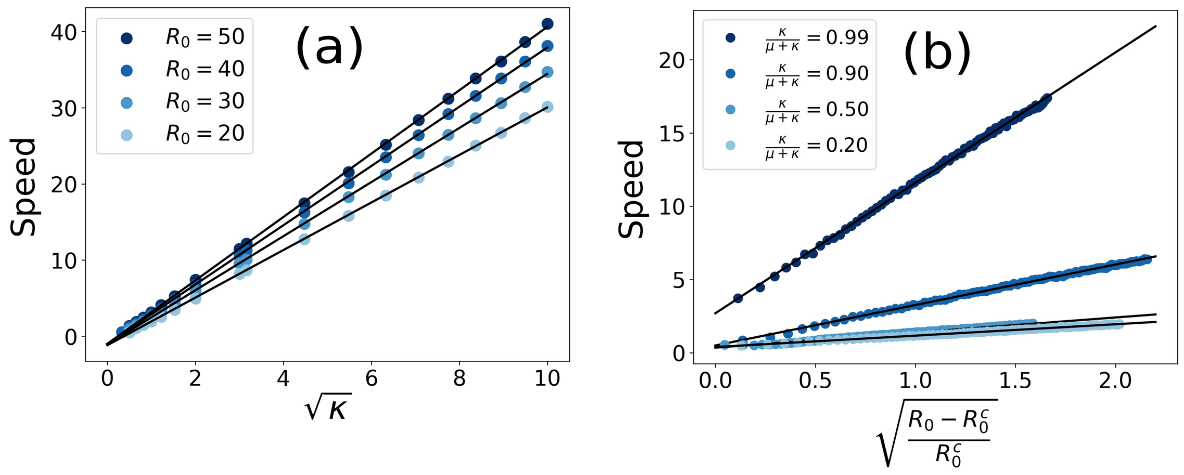
\includegraphics[width=1\textwidth]{Figures/Front_velocity.png}
    \caption[
        Analysis of the spreading speed of the infected population
    ]{(a) Disease spreading speed as function of the square root of
        the parasite mobility for several values of $R_0$. The plot shows a
        remarkable
        agreement with \cref{eq:front_vel}. (b) Disease spreading speed as
        function of
        the square root of the distance to the critical value of $R_0$ for
        several
        values of the parasite mobility.}
    \label{fig:front_velocity}
\end{figure}

The extinction time is defined as the time elapsed from the beginning of
the epidemic until the system reaches its absorbing state, that is, when no
parasites or infected individuals are left. From \cref{eq:front_vel}, we expect
the time to extinction to increase when the parasite mobility is decreased.
Moreover, we expect the extinction time to decrease with the distance to the
epidemic threshold, as we expect to reach faster the absorbing state for larger
values of the spatial basic reproduction number.

In the limiting case where all (or almost all) hosts die, it is clear that
the disease must have spread to the entire system. Thus, in this limit, the
extinction time should be proportional to the inverse of the disease spreading
speed, $t_{\textrm{ext}}\sim 1/v$. Then, in this limit, we can relate the
extinction time with the parasite mobility as follows,
\begin{equation}\label{eq:t_ext}
    t_{\textrm{ext}}\sim\frac{1}{\sqrt{\kappa}} \quad \textrm{for} \quad
    \tilde{R}_0\gg1 \ .
\end{equation}
However, the absorbing state is not always reached after all hosts becoming
infected and \cref{eq:t_ext} is only expected to work far from the epidemic
threshold, when the disease is expected to spread to the entire system.

In \cref{fig:extinction_time}(a) the extinction time is plotted against the
basic reproduction number for some values of the parasite mobility. As
expected, the extinction time increases for lower values of the parasite
mobility. The increasing behaviour before the peak can be understood as the
increasing time needed for the initial perturbations to decay to the
disease-free phase. After the peak, the greater the basic reproduction number
the faster the epidemic will reach its absorbing state with a non-negligible
number of dead individuals. So, with this interpretation, the peaks of the
extinction time should coincide with the epidemic threshold for each value of
the parasite mobility.

\begin{figure}[H]
    \centering
    \includegraphics[width=\textwidth]{Figures/Extinction_time.png}
    \caption[
        Analysis of the extinction time of the epidemic]{(a) Extinction time
        for some values of the parasite mobility.
        (b) Comparison of the critical $R_0$ value computed with
        \cref{eq:R_0ibm}
        compared to the values obtained numerically by computing the maximum of
        the
        extinction time. (c) Scaling of the extinction time with several values
        of the
        parasite mobility. (d) Representation of the square of the extinction
        time as
        function of the inverse of the parasite mobility. The inset shows the
        zone
        where this relation has been computed, showing a good agreement with
        \cref{eq:t_ext}.}
    \label{fig:extinction_time}
\end{figure}

In \cref{fig:extinction_time}(b) we compare the numerical value of $R_0$ at
which the extinction time peaks with the theoretical value of $R_0^c$, computed
with \cref{eq: threshold_corrections}, showing good agreement. Thus, the
dependence of the extinction time with $R_0$ should vanish if plotted against
the distance to $R_0^c$. Furthermore, if the extinction time is normalised
(dividing each line by its maximum), all the lines should collapse near the
transition point. In \cref{fig:extinction_time}(c) the normalised extinction
time is plotted against the distance to the critical value of $R_0$. The
scaling is shown to be valid only near the transition point, as expected.

In the limiting case where the epidemic dies by infecting a large part of
the host population, i.e. for a large enough $R_0$ value, the extinction time
should follow \cref{eq:t_ext}, as previously discussed. In
\cref{fig:extinction_time}(d) we show how the extinction time relates to the
parasite mobility in this limit, following the predicted behaviour.

\section{Conclusions} \label{sec: conclusions}

In this work we have developed a spatially-explicit individual-based model
for parasite-produced marine epidemics of immobile hosts. This study has
allowed us to tackle important questions in marine epidemiology, as how spatial
constraints affect epidemic spreading in filter-feeder populations or how will
the infected population of hosts change in space and time. While addressing the
aforementioned questions, we have shown that there exists a regime of high
parasite mobility where the time progression of both host and parasite
populations can be well described by the non-spatial version of the model (i.e.
the system of ODE's presented in \cite{GimenezRomero2021}). We have also shown
that a fast-slow approximation for the time progression of the parasite
population, already presented in \cite{GimenezRomero2021}, can be extended for
spatial systems. Interestingly, the conditions under which this approximation
is valid  are less restrictive than in the non-spatial case, and regimes in
which this approximation is valid for low mobility and comparable time scales
are reported in this contribution.

We have derived an approximate analytical expression of the
\textit{spatial} basic reproduction number, that allows to predict the onset of
a global epidemic in a spatial model. The obtained expression explicitly shows
a trade-off between the intrinsic pathosystem dynamics (i.e. $R_0$) and a
factor accounting for parasite mobility. Moreover, the spatial threshold
defined by $\tilde{R}_0=1$ separates the final state of the system in two
different phases, namely a disease-free phase and a propagation phase. In the
propagation phase, any initial condition of infected individuals or parasites
will propagate throughout the system, causing a proper outbreak. On the other
hand, in the disease-free phase the conditions are not sufficient for a local
introduction of parasites or infected individuals to spread through the system.
The effect of the parasite mobility in the spatial basic reproduction number is
clear, the more parasites move the more infections they cause.

The spatiotemporal behaviour of the system has been investigated in the
propagation phase. First, we showed that the infected population spreads
through the space with a speed directly proportional to the square root of the
diffusion coefficient of parasites, showing good agreement between the derived
analytical expression and numerical simulations. The time to extinction has
been also studied by means of numerical simulations, showing that, if the
system is far above enough of the spatial threshold, the time to extinction can
be analytically computed, in good agreement with simulations. We obtained that
larger values of the parasite mobility yield more severe epidemics in which
there are more infections and the extinction is faster.

To summarise, in the present work we have introduced and analysed and
Individual-Based approach to epidemic transmission in spatially extended
systems of immobile hosts. The infection mechanism is due to mobile parasites,
that are in turn produced by infected hosts. The study allows to answer some
biologically relevant questions, like predicting the occurrence of a global
epidemic outbreak or its velocity of expansion through the system. Thus, the
analytical and computational results of the model shed light on the underlying
mechanisms underpinning the emergence of a global epidemic outbreak and its
spatial progression. This work provides a first step into the spatial-explicit
individual-based modelling of marine epidemics of immobile hosts.

Although this work has considered the case of a spatially homogeneous
distribution of hosts, we plan to extend the study to more general cases,
discussing the effect of inhomogeneous spatial host distributions. Furthermore,
other biological relevant effects could be added to the model to enhance the
description of different epidemics, e.g. infected individuals could still
filter parasites or parasite-load dependent infection process. The model could
also describe epidemics on other immobile species such as filter feeders like
sponges or other bivalves, corals, intertidal communities or starfishes
provided that the necessary modifications in the model are properly included.
Stochastic spatially-explicit descriptions like the one presented here could be
also extended to the study of epidemics of other immobile hosts, like
vector-borne diseases of plants. However, this would imply a quite different
model to describe the different epidemic compartments of the vectors and also
their ecological features. We hope these studies can be useful in conservation
plans or ecosystem management and could serve as a basis for more sophisticated
models.